\RequirePackage{fix-cm}
\documentclass[10pt,letterpaper]{article}
\usepackage[margin=0.48in,top=0.46in,bottom=0.65in,footskip=24pt]{geometry}
\usepackage{fontspec,amsmath,amssymb,array,tabularx,fancyhdr,xcolor,hyperref,enumitem,tikz}
\setmainfont{Latin Modern Sans}\setsansfont{Latin Modern Sans}
\definecolor{Accent}{HTML}{225D68}\definecolor{Muted}{HTML}{4D555B}
\hypersetup{hidelinks,pdftitle={Thermodynamics B 2027 — Exam reference},pdfauthor={Greg Hogan and the soso contributors}}
\input{@@NOTICE@@}
\pagestyle{fancy}\fancyhf{}\renewcommand{\headrulewidth}{0pt}
\fancyfoot[L]{\sffamily\fontsize{6.3}{8}\selectfont\sosocredit}
\fancyfoot[R]{\sffamily\fontsize{8}{9}\selectfont\thepage\,/\,6}
\renewcommand{\footrulewidth}{0.3pt}
\setlength{\parindent}{0pt}\setlength{\parskip}{4pt}\setlength{\emergencystretch}{12pt}
\setlist[itemize]{leftmargin=12pt,itemsep=1pt,topsep=2pt,parsep=0pt}
\setlength{\tabcolsep}{3pt}\renewcommand{\arraystretch}{1.15}
\newcommand{\head}[2]{\hypertarget{p\thepage}{} {\sffamily\bfseries\fontsize{13}{15}\selectfont THERMODYNAMICS B}\hfill{\sffamily\fontsize{8.5}{10}\selectfont 2027\quad|\quad EXAM REFERENCE}\par\vspace{2pt}\hrule height0.6pt\vspace{4pt}{\sffamily\bfseries\fontsize{10.3}{12}\selectfont #1}\par{\sffamily\fontsize{7.4}{9}\selectfont #2}\par\vspace{3pt}}
\newcommand{\sect}[1]{\par\vspace{5pt}{\sffamily\bfseries\color{Accent}\fontsize{10.2}{11}\selectfont #1}\par\vspace{2pt}{\color{Accent}\hrule height0.35pt}\vspace{3pt}}
\newcommand{\eq}[1]{\par\vspace{1pt}\(\displaystyle #1\)\par\vspace{1pt}}
\newcommand{\term}[2]{\textbf{#1}\enspace #2\par}
\newcommand{\trap}[1]{\textbf{Watch for:} #1\par}
\newenvironment{cols}{\begin{minipage}[t]{0.482\textwidth}\raggedright}{\end{minipage}}
\newcommand{\nextcol}{\end{minipage}\hfill\begin{minipage}[t]{0.482\textwidth}\raggedright}
\begin{document}
\fontsize{10.5}{12.6}\selectfont
\head{1 · Start with quantities and units}{Quick lookup: \hyperlink{p2}{materials / phases 2} · \hyperlink{p3}{heat transfer 3} · \hyperlink{p4}{gases / laws 4} · \hyperlink{p5}{engines / people 5} · \hyperlink{p6}{device / scoring 6}}
\begin{cols}
\sect{Choose the system}
\term{System}{The matter or region being studied. Surroundings are everything outside it; the boundary defines what can cross.}
\begin{tabularx}{\linewidth}{@{}l>{\raggedright\arraybackslash}X@{}}
\textbf{Type}&\textbf{Can cross the boundary}\\\hline
Open&Mass and energy.\\
Closed&Energy, but not mass.\\
Isolated&Neither mass nor energy (idealization).\\
\end{tabularx}
\term{Intensive}{Independent of amount: temperature, pressure, density, specific heat.}
\term{Extensive}{Scales with amount: mass, volume, internal energy, heat capacity. Doubling the sample doubles these, not its temperature.}
\sect{Heat is a transfer, not a substance}
\term{Temperature $T$}{Property determining thermal equilibrium and the direction of spontaneous heat flow. For an ideal gas, it tracks mean translational kinetic energy.}
\term{Heat $Q$}{Energy crossing a boundary because of a temperature difference. Net heat flows hot $\to$ cold without external work.}
\term{Internal energy $U$}{Microscopic kinetic and potential energy stored within a system. It is not the same as temperature or the system's bulk motion.}
\term{Zeroth law}{If A and B are separately in thermal equilibrium with C, then A and B are in thermal equilibrium with each other. This makes thermometers possible.}
\trap{Equal temperatures do not imply equal internal energies. A lake and a cup can share $T$ but have very different energy stores.}
\sect{Temperature conversion}
\eq{T_{\mathrm K}=T_{^\circ\mathrm C}+273.15}
\eq{T_{^\circ\mathrm F}=\tfrac95T_{^\circ\mathrm C}+32}
\eq{T_{^\circ\mathrm C}=\tfrac59(T_{^\circ\mathrm F}-32)}
\eq{\Delta T_{\mathrm K}=\Delta T_{^\circ\mathrm C}
\quad;\quad \Delta T_{^\circ\mathrm F}=\tfrac95\Delta T_{^\circ\mathrm C}}
An interval of $10\,^{\circ}$C is $10$ K, not $283.15$ K. Use absolute kelvin in gas laws, radiation and temperature ratios.
\nextcol
\sect{Units and useful constants}
\begin{tabularx}{\linewidth}{@{}l>{\raggedright\arraybackslash}X@{}}
\textbf{Quantity}&\textbf{SI unit / relation}\\\hline
Energy, heat, work&joule: $1\,\mathrm J=1\,\mathrm{N\,m}$\\
Power $P$&watt: $1\,\mathrm W=1\,\mathrm{J/s}$\\
Pressure $p$&pascal: $1\,\mathrm{Pa}=1\,\mathrm{N/m^2}$\\
Volume&$1\,\mathrm L=10^{-3}\,\mathrm{m^3}$\\
&$1\,\mathrm{mL}=1\,\mathrm{cm^3}=10^{-6}\,\mathrm{m^3}$\\
Heat unit&$1\,\mathrm{cal}=4.184\,\mathrm J$ (thermochemical)\\
Food Calorie&$1\,\mathrm{Cal}=1\,\mathrm{kcal}=4184\,\mathrm J$\\
Atmosphere&$1\,\mathrm{atm}=101325\,\mathrm{Pa}$\\
Gas constant&$R=8.314\,\mathrm{J/(mol\,K)}$\\
Boltzmann constant&$k_{\mathrm B}=1.381\times10^{-23}\,\mathrm{J/K}$\\
Avogadro constant&$N_{\mathrm A}=6.022\times10^{23}\,\mathrm{mol^{-1}}$\\
\end{tabularx}
\sect{Water near ordinary conditions}
\eq{\rho\approx1.00\,\mathrm{g/mL}\qquad
 c\approx4.18\,\mathrm{J/(g\,K)}}
At $1$ atm: melting near $0\,^{\circ}$C and boiling near $100\,^{\circ}$C. These are pressure-dependent, not universal phase boundaries.

Useful approximations: ice $c\approx2.1\,\mathrm{J/(g\,K)}$; water fusion $L_f\approx334\,\mathrm{J/g}$; vaporization at $100\,^{\circ}$C $L_v\approx2260\,\mathrm{J/g}$. Use problem-supplied values when given.
\sect{Fast quantitative checks}
\eq{P=\frac{E}{t}\qquad\rho=\frac{m}{V}\qquad p=\frac{F}{A}}
\textbf{Geometry:} circle $A=\pi r^2$; cylinder $V=\pi r^2h$; rectangular box $V=abc$; sphere $A=4\pi r^2$, $V=\frac43\pi r^3$. Convert dimensions \emph{before} squaring or cubing.

\textbf{Method:} define system $\to$ list knowns with units $\to$ choose assumptions $\to$ rearrange formula $\to$ substitute $\to$ check sign, units and magnitude. Keep guard digits; round the final answer to justified precision.
\trap{Use seconds with watts; kilograms with $\mathrm{J/(kg\,K)}$, grams with $\mathrm{J/(g\,K)}$.}
\end{cols}
\newpage
\head{2 · Heating, phase changes and mixing}{Use $mc\Delta T$ within one phase; use $mL$ during a phase change.}
\begin{cols}
\sect{Heat capacity versus specific heat}
\eq{C=\frac{Q}{\Delta T}\qquad c=\frac{Q}{m\Delta T}\qquad C=mc}
\term{Heat capacity $C$}{Energy per temperature change for a whole object; unit J/K.}
\term{Specific heat $c$}{Energy per mass per temperature change; unit J/(kg K) or J/(g K).}
\eq{Q=mc(T_f-T_i)}
Assumes no phase change and approximately constant $c$ over the interval. Cooling gives $Q<0$ under a heat-into-sample sign convention.

\textbf{Fast water calculation:} $100$ mL water has $m\approx100$ g and $C\approx418$ J/K. A $5\,^{\circ}$C rise stores about $2090$ J in the water. It does \emph{not} measure all energy emitted by the lamp.
\sect{Phase changes}
\begin{tabularx}{\linewidth}{@{}l>{\raggedright\arraybackslash}X@{}}
\textbf{Energy absorbed}&\textbf{Reverse releases energy}\\\hline
Melting: solid $\to$ liquid&Freezing\\
Vaporization: liquid $\to$ gas&Condensation\\
Sublimation: solid $\to$ gas&Deposition\\
\end{tabularx}
\eq{|Q|=mL}
Here $L$ is positive latent heat per mass. Choose the sign from direction. For a pure substance changing phase at fixed pressure, energy can change with no temperature change.

\textbf{Evaporation} occurs at a surface below boiling; escaping energetic molecules can cool the remaining liquid. \textbf{Boiling} occurs throughout a liquid when its vapor pressure equals external pressure.
\sect{Heating curve: add the stages}
\begin{center}
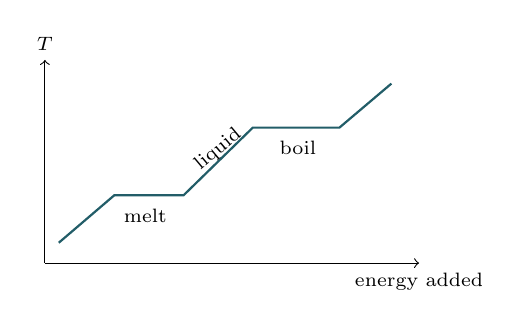
\begin{tikzpicture}[x=0.44cm,y=0.43cm,font=\scriptsize]
\draw[->] (0,0)--(10.8,0) node[below]{energy added};
\draw[->] (0,0)--(0,6) node[above]{$T$};
\draw[thick,Accent] (.4,.6)--(2,2)--(4,2)--(6,4)--(8.5,4)--(10,5.3);
\node at (2.9,1.4){melt};\node at (7.3,3.4){boil};
\node[rotate=40] at (5.0,3.35){liquid};
\end{tikzpicture}
\end{center}
Slopes: $mc\Delta T$. Flat segments: $mL$. At constant input power, time on each stage is $|Q|/P$; greater heat capacity makes the temperature slope gentler.
\nextcol
\sect{An energy-accounting recipe}
For an insulated mixing problem with no external work:
\eq{\sum_i Q_i=0}
Use signed $Q_i=m_i c_i(T_f-T_i)$ for objects that stay in one phase. Include the container if its heat capacity matters. Objects share the final equilibrium temperature, not equal heat changes.

For two samples with no phase change or loss:
\eq{T_f=\frac{m_1c_1T_1+m_2c_2T_2}{m_1c_1+m_2c_2}}
\textbf{Check:} $T_f$ lies between the initial temperatures. The larger $mc$ pulls $T_f$ closer to its own initial temperature.

\textbf{Example:} mix $50$ g of $80\,^{\circ}$C water with $100$ g of $20\,^{\circ}$C water; negligible container/loss. Same $c$ cancels:
\eq{T_f=\frac{50(80)+100(20)}{150}=40\,^{\circ}\mathrm C}
\sect{When ice or steam is involved}
Do not jump directly to the weighted-average formula.
\begin{itemize}
\item Compute energy needed to reach a phase boundary.
\item Compute the latent-heat requirement.
\item Compare with energy available from the other sample.
\item If insufficient to finish the transition, solve the amount melted/condensed; phase coexistence fixes $T_f$ at the boundary (fixed pressure).
\item Only leftover energy can warm/cool the new phase.
\end{itemize}
\textbf{Example:} $10$ g ice at $0\,^{\circ}$C requires $3340$ J to melt completely. Adding only $1000$ J melts about $3.0$ g; the mixture remains near $0\,^{\circ}$C at 1 atm.
\sect{Read a phase diagram}
Axes are \textbf{pressure versus temperature}, not energy versus temperature. Each region is one phase; boundary curves show coexistence.
\term{Triple point}{Three phases coexist at one pressure and temperature.}
\term{Critical point}{End of the liquid--gas coexistence curve. Above the critical temperature, compression does not produce a distinct liquid--gas transition.}
\term{Path matters}{At constant pressure move horizontally on a diagram with $T$ horizontal. At constant temperature move vertically. Read axes first.}
Water's solid--liquid boundary slopes differently from that of most substances: ordinary ice is less dense than liquid water, so increasing pressure can favor melting near that boundary.
\end{cols}
\newpage
\head{3 · Heat transfer and radiation}{Core: mechanisms and material response. State/National extension: blackbodies and radiant exitance.}
\begin{cols}
\sect{Three transfer routes}
\term{Conduction}{Energy transfer through microscopic interactions without bulk transport of matter. Important in solids and still fluids.}
\term{Convection}{Energy carried by bulk fluid motion. Natural convection arises from buoyancy; forced convection uses a fan or pump.}
\term{Radiation}{Transfer by electromagnetic waves; no material medium required. Can cross a vacuum.}
They can act simultaneously. A vacuum suppresses conduction/convection across the gap, but not radiation.
\sect{Conduction through a slab}
For steady one-dimensional flow through a uniform slab:
\eq{P=\frac{Q}{t}=kA\frac{T_h-T_c}{L}}
$k$: thermal conductivity, W/(m K); $A$: area normal to flow, m$^2$; $L$: thickness, m. Larger $k$, area or temperature difference increases the rate; larger thickness decreases it.

\textbf{Compare:} double thickness $\Rightarrow$ half the rate, if the other quantities stay fixed. Real assemblies also have contact and surface resistances.
\trap{Conductivity $k$ describes transfer rate; specific heat $c$ describes stored energy per mass and temperature change. They are not interchangeable.}
\sect{Convection and insulation}
A warmed fluid often expands, becomes less dense and rises; cooler fluid replaces it. Gravity and geometry matter. Heating from above can produce stable temperature layering rather than vigorous mixing.

Trapped air can insulate because air conducts poorly and small pockets limit circulation. A draft carries warm air away. A reflective surface acts mainly on radiation, not automatically on convection.

\textbf{Useful comparison model:}
\eq{P_{\mathrm{conv}}=hA(T_s-T_{\mathrm{air}})}
$h$ is a condition-dependent heat-transfer coefficient, not a universal material constant. Use only if provided or measured; airflow changes it.
\sect{Lamp collector: follow the path}
Lamp radiation $\to$ absorbing surface $\to$ cup/water. Energy also warms the apparatus and escapes to the surroundings. Improve absorption, useful thermal contact and loss control; verify the net result with trials.
\nextcol
\sect{Absorb, reflect or transmit}
For incident radiant energy at a specified wavelength:
\eq{\alpha+\rho_r+\tau=1}
$\alpha$: absorptance; $\rho_r$: reflectance; $\tau$: transmittance. For an opaque surface, $\tau=0$.

Dark appearance concerns visible light. A surface's behavior in infrared can differ; a transparent cover can transmit visible light while interacting differently with longer wavelengths. Do not infer full thermal performance from color alone.

A good thermal emitter is a good absorber under matching wavelength/direction and equilibrium conditions. Shiny low-emissivity surfaces tend to reflect thermal radiation.
\sect{Blackbody \hfill\small State / National}
An ideal blackbody absorbs all incident radiation. Its emitted spectrum depends only on its temperature. Heating it increases total emission and shifts the peak toward shorter wavelengths.

Real surfaces have emissivity $0\leq\varepsilon\leq1$. The graybody approximation treats $\varepsilon$ as constant over the relevant spectrum.
\sect{Radiant exitance \hfill\small State / National}
Radiant exitance $M$ is emitted power per surface area, in W/m$^2$; it is not total power.
\eq{M_{\mathrm{blackbody}}=\sigma T^4\qquad M=\varepsilon\sigma T^4}
\eq{P_{\mathrm{emit}}=\varepsilon\sigma A T^4}
\eq{\sigma=5.670\times10^{-8}\,\mathrm{W\,m^{-2}\,K^{-4}}}
For a small gray object exchanging radiation with large uniform surroundings (appropriate view/geometry assumptions):
\eq{P_{\mathrm{net,out}}=\varepsilon\sigma A(T_s^4-T_{\mathrm{sur}}^4)}
\textbf{Checks:} zero net exchange at equal temperatures; net inward when surroundings are hotter. Use kelvin and emitting area, not Celsius or just the illuminated footprint.

\textbf{Scaling:} doubling absolute $T$ multiplies emitted power by $16$ if $A$ and $\varepsilon$ stay fixed. This is \emph{not} a doubling of Celsius temperature.
\trap{A bulb's electrical rating is not power absorbed by the water. Do not assume a reflector lamp at short distance obeys a simple point-source inverse-square prediction; calibrate the actual setup.}
\end{cols}
\newpage
\head{4 · Gases, work and the thermodynamic laws}{Sign convention used here: $Q>0$ enters the system; $W>0$ is work done by the system.}
\begin{cols}
\sect{Ideal gas relations}
\eq{pV=nRT=Nk_{\mathrm B}T\qquad N=nN_{\mathrm A}}
Use \textbf{absolute pressure}, kelvin and matching units. $n$ is amount in moles, not mass. SI: Pa, m$^3$, J/(mol K).
\eq{p_{\mathrm{absolute}}=p_{\mathrm{gauge}}+p_{\mathrm{ambient}}}
For fixed amount of ideal gas:
\eq{\frac{p_1V_1}{T_1}=\frac{p_2V_2}{T_2}}
\begin{tabularx}{\linewidth}{@{}l>{\raggedright\arraybackslash}X@{}}
\textbf{Held fixed}&\textbf{Relationship}\\\hline
$T,n$&$pV=$ constant (Boyle)\\
$p,n$&$V/T=$ constant (Charles)\\
$V,n$&$p/T=$ constant\\
$p,T$&$V\propto n$\\
\end{tabularx}
\textbf{Example:} a sealed rigid ideal-gas container warms from $300$ K to $330$ K. Its absolute pressure rises by a factor $330/300=1.10$.
\trap{The model is least reliable near condensation and at high density. A gas does not have particles all moving at one speed.}
\sect{First law: energy accounting}
\eq{\Delta U=Q-W}
If a question uses work \emph{on} the system instead, write $\Delta U=Q+W_{\mathrm{on}}$ and do not mix the conventions.

\textbf{Examples:} $Q=500$ J enters and gas does $200$ J work: $\Delta U=300$ J. Adiabatic compression with $W=-200$ J gives $\Delta U=+200$ J.
\sect{Work and a $p$--$V$ graph}
For expansion against constant external pressure:
\eq{W=p_{\mathrm{ext}}(V_f-V_i)}
Work is the area under the pressure--volume path when the plotted pressure is the relevant boundary pressure; the usual equilibrium $p$--$V$ picture assumes a quasistatic process.

Expansion $\Rightarrow W>0$; compression $\Rightarrow W<0$. For a cycle, net work is the enclosed signed area. A clockwise cycle is net work output. No calculus is needed for rectangular or other simple-area paths.
\nextcol
\sect{Four process models}
\begin{tabularx}{\linewidth}{@{}>{\raggedright\arraybackslash}p{0.27\linewidth}>{\raggedright\arraybackslash}X@{}}
\textbf{Process}&\textbf{Constraint and consequence}\\\hline
Isothermal&Constant $T$. For an ideal gas, $\Delta U=0$, so $Q=W$. Heat may flow.\\
Adiabatic&No heat transfer, $Q=0$, so $\Delta U=-W$. Temperature can change.\\
Isochoric&Constant $V$; no boundary expansion work, so $Q=\Delta U$ if no other work occurs.\\
Isobaric&Constant $p$; boundary work $W=p\Delta V$. Heat can both change $U$ and do work.\\
\end{tabularx}
For an ideal gas, internal energy depends only on $T$. This does not mean $U$ depends only on $T$ for every real substance.

\textbf{On a $p$--$V$ graph:} isochoric is vertical; isobaric is horizontal; isothermal ideal gas satisfies $p\propto1/V$. An adiabatic expansion cools an ideal gas and is steeper than an isothermal expansion from the same state (reversible ideal-gas comparison).
\sect{Second law: direction and limits}
\begin{itemize}
\item Heat does not spontaneously flow from colder to hotter without other changes/work.
\item A cyclic heat engine cannot turn all heat from a single reservoir into net work.
\item Total entropy of an isolated system does not decrease. It stays constant in an ideal reversible process and increases in an irreversible one.
\end{itemize}
Entropy measures energy dispersal and the multiplicity of compatible microscopic states. It is not simply a synonym for visible mess. A subsystem's entropy may decrease if its surroundings compensate.
\sect{Third law \hfill\small State / National}
The entropy of a perfect crystal approaches zero as its temperature approaches $0$ K. A related unattainability formulation says absolute zero cannot be reached through a finite sequence of cooling processes.

Do not replace this with ``all microscopic motion stops'': quantum behavior makes that claim too broad. The first law concerns conservation; the third concerns the low-temperature limit.
\end{cols}
\newpage
\head{5 · Engines, cycles and the people behind the ideas}{Positive heat magnitudes $Q_h$ and $Q_c$ refer to heat taken from the hot reservoir and rejected to the cold one.}
\begin{cols}
\sect{A heat engine must reject heat}
A cyclic engine returns to its initial internal energy: $\Delta U_{\mathrm{cycle}}=0$.
\eq{W_{\mathrm{net}}=Q_h-Q_c}
\eq{\eta=\frac{W_{\mathrm{net}}}{Q_h}=1-\frac{Q_c}{Q_h}}
Efficiency is dimensionless; multiply by $100\%$ for percentage. The denominator is \emph{heat supplied}, not heat rejected or net work.

\begin{center}
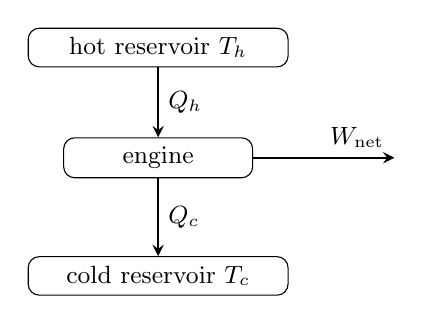
\begin{tikzpicture}[font=\small,>=stealth]
\node[draw,rounded corners,minimum width=3.3cm] (h) at (0,2.2) {hot reservoir $T_h$};
\node[draw,rounded corners,minimum width=2.4cm] (e) at (0,0.8) {engine};
\node[draw,rounded corners,minimum width=3.3cm] (c) at (0,-0.7) {cold reservoir $T_c$};
\draw[->,thick] (h)--node[right]{$Q_h$}(e);
\draw[->,thick] (e)--node[right]{$Q_c$}(c);
\draw[->,thick] (e.east)--(3,0.8) node[above left]{$W_{\mathrm{net}}$};
\end{tikzpicture}
\end{center}
\textbf{Example:} an engine absorbs $1000$ J and rejects $650$ J each cycle. Work is $350$ J; efficiency is $0.35=35\%$.
\sect{Carnot limit}
Between reservoirs at absolute temperatures $T_h>T_c$:
\eq{\eta\leq\eta_{\mathrm C}=1-\frac{T_c}{T_h}}
Equality describes an ideal reversible engine. Real irreversibility reduces efficiency. Raise $T_h$ or lower $T_c$ to raise the theoretical limit; kelvin is essential.

\textbf{Example:} $T_h=500$ K, $T_c=300$ K gives $\eta_{\mathrm C}=40\%$. This is an upper bound, not a promise for an actual device.
\sect{Refrigerator versus heat pump}
Both use work to move heat from cold to hot:
\eq{Q_h=Q_c+W_{\mathrm{in}}}
A refrigerator's useful effect is removing $Q_c$; a heat pump's is delivering $Q_h$. A coefficient of performance can exceed 1 because it compares \emph{heat moved} with work input; it is not heat-engine efficiency.
\eq{\mathrm{COP}_{\mathrm{ref}}=\frac{Q_c}{W_{\mathrm{in}}}\qquad
\mathrm{COP}_{\mathrm{hp}}=\frac{Q_h}{W_{\mathrm{in}}}}
\nextcol
\sect{Eight names, eight connections}
\term{Joseph Black}{Specific heat and latent heat: warming a material and changing its phase require different energy accounting.}
\term{James Prescott Joule}{Mechanical work and thermal energy are quantitatively equivalent; experiments helped establish energy conservation.}
\term{Sadi Carnot}{Ideal cyclic heat engines and the limits imposed by hot and cold reservoir temperatures.}
\term{William Thomson (Lord Kelvin)}{Absolute thermodynamic temperature scale and foundational work on thermodynamics. Use kelvin for absolute-temperature comparisons.}
\term{Rudolf Clausius}{Second-law formulations and the concept of entropy: direction and irreversible change, not only conservation.}
\term{James Clerk Maxwell}{Statistical treatment of gases and a distribution of molecular speeds; macroscopic properties arise from particle behavior.}
\term{Ludwig Boltzmann}{Statistical mechanics connecting entropy with the number of microscopic arrangements compatible with a state.}
\term{Max Planck}{Blackbody radiation and quantized energy exchange, an essential step toward quantum physics.}
\sect{Separate the questions}
\begin{tabularx}{\linewidth}{@{}l>{\raggedright\arraybackslash}X@{}}
\textbf{Question}&\textbf{First place to look}\\\hline
What temperature?&Equilibrium; zeroth law\\
How much energy?&First law; $mc\Delta T$; $mL$\\
How fast?&Power and transfer mechanisms\\
Which direction?&Second law; total entropy\\
Best possible engine?&Carnot limit\\
Absolute-zero limit?&Third law\\
\end{tabularx}
\sect{Last-pass error check}
\begin{itemize}
\item Did I distinguish heat from internal energy?
\item Did I use kelvin for a ratio or fourth power?
\item Is there a phase change hidden in the problem?
\item Does my work sign match my convention?
\item Is this an ideal model or an actual measured device?
\item Are all assumptions and units stated?
\end{itemize}
\end{cols}
\newpage
\head{6 · Device testing, prediction and scoring}{2027 B: heat 100 mL of water with the supplied lamp. Use your own calibration data alongside this reference.}
\begin{cols}
\sect{Fast tournament checklist}
\textbf{Bring:} room-temperature device and spares for impound; permitted tools; organized paper notes/graphs; up to two Class III calculators. Paper references have no numerical page limit. Tools and paper notes are not impounded.

\textbf{Device:} complete assembly including supplied cup must fit a $30.0$ cm cube. Use the clear 9 oz cup unaltered and removable, without attached fasteners or adhesives. No part may touch the water and nothing may be added. No energy sources, electrical components, thermometers/probes, commercial thermoses/coolers or vacuum-sealed devices. Hazardous materials are prohibited, including polystyrene. Glass is allowed; the November clarification calls for caution and Category C goggles while interacting with glass-containing devices. Tongs, hot pads and heat-resistant gloves are permitted.

\textbf{Lamp height:} table to bulb's bottommost point. Regionals: $40,45,50$ cm; States: $40,45,50,55$ cm; Nationals: $40$--$65$ cm in $1$ cm steps. Heating: $10$ min Regionals; $10$--$15$ min in whole-minute steps States/Nationals. Supervisor assigns conditions.

\textbf{Sequence:} 3 min setup/modification $\to$ receive cup and reported starting $T$ $\to$ up to 1 min cup insertion $\to$ hands off during heating $\to$ submit final-$T$ prediction \emph{before heating ends} $\to$ remove cup completely for measurement, aiming within 1 min after lamp-off.

Cup insertion/removal may involve clarified lid/door and orientation/position actions, not unrelated modifications. Do not swirl, shake or stir water. The supervisor measures start/final temperatures with the same thermometer for that team; no probe remains in the device.
\sect{Prediction from evidence}
Record lamp geometry/specifications, room and initial water temperature, heating time, cup and device configuration. Use repeated trials under matched conditions. Keep the final measurement procedure consistent with competition.

\textbf{Interpolate, do not guess:} between neighboring measurements $(x_1,T_1)$ and $(x_2,T_2)$:
\eq{T(x)\approx T_1+\frac{x-x_1}{x_2-x_1}(T_2-T_1)}
This is a local empirical approximation. Do not extrapolate far or vary height/time while pretending other conditions are fixed. Report trial spread; reserve independent trials to test predictions.
\nextcol
\sect{Score components}
Use Celsius for \emph{all official scoring calculations}. Let $E$ be exam points and ``best'' the highest corresponding value among teams.
\eq{\mathrm{TG}=\max(0,T_{\mathrm{final}}-T_{\mathrm{start}})}
\eq{\mathrm{ES}=50\frac{E}{E_{\mathrm{best}}}\qquad
\mathrm{TS}=30\frac{\mathrm{TG}}{\mathrm{TG}_{\mathrm{best}}}}
\eq{\mathrm{PE}=\max\!\left(0,1-\frac{|T_{\mathrm{final}}-T_{\mathrm{pred}}|}{T_{\mathrm{final}}}\right)}
\eq{\mathrm{PS}=20\frac{\mathrm{PE}}{\mathrm{PE}_{\mathrm{best}}}\qquad
\mathrm{FS}=\mathrm{ES}+\mathrm{TS}+\mathrm{PS}}
PE divides by final \emph{Celsius temperature}, not temperature gain or kelvin. If final $T=40\,^{\circ}$C and prediction $=38\,^{\circ}$C, PE $=0.95$. With best PE $=1$, PS $=19$.

For each competition violation multiply TS and PS by $0.9$; for each construction violation remaining after setup multiply them by $0.7$. Explicit zeros take precedence: prohibited energy sources or touching during heating zero TS and PS; late prediction zeros PS. Missing impound is a construction violation under the clarification. Ties: TS, then ES, then selected exam questions.
\sect{Prediction sanity checks}
$100$ mL water needs about $418$ J per $1\,^{\circ}$C rise. Net storage of $1$ W in water for $600$ s gives about $1.44\,^{\circ}$C rise. This assumes that watt is \emph{net power into water}, not the lamp rating. Actual heating can curve as losses grow; do not assume constant slope.
\sect{Scope and source trail}
Written test: systems/temperature; phases/gases; transfer/materials; processes/laws/engines; eight scientists. State/National also add blackbodies, radiant exitance, Stefan--Boltzmann and third law. No required trigonometry or calculus.

{\footnotesize Original summary based on the supplied 2027 B manual, B56--B58; \href{https://www.soinc.org/book/export/html/222}{official Thermodynamics clarifications}; \href{https://www.soinc.org/events/rules-corrections}{rules corrections}; and OpenStax \href{https://openstax.org/books/college-physics-2e/pages/13-introduction-to-temperature-kinetic-theory-and-the-gas-laws}{College Physics 2e, chapters 13--15}. Science/history source details accompany the study guide. Rules checked 17 Nov 2026. Official rules and subsequent updates control; this is a retrieval aid, not a replacement.}
\end{cols}
\end{document}
